% Figure 5.13: IDP Database ER Diagram
% Professional ER Diagram with Crow's Foot Notation
% Compile with: pdflatex fig_5_13_er_diagram.tex

\documentclass[border=15pt]{standalone}
\usepackage{tikz}
\usetikzlibrary{shapes.geometric, arrows.meta, positioning, calc, decorations.markings}
\usepackage{xcolor}

% Professional academic color scheme (muted grayscale)
\definecolor{entityHeader}{RGB}{70, 130, 180}    % Steel blue
\definecolor{entityBody}{RGB}{245, 245, 245}     % Light gray
\definecolor{pkColor}{RGB}{119, 136, 153}        % Light slate gray
\definecolor{fkColor}{RGB}{105, 105, 105}        % Dim gray
\definecolor{lineColor}{RGB}{33, 33, 33}         % Dark text
\definecolor{textdark}{RGB}{33, 33, 33}

% Crow's foot notation styles
\tikzset{
    % One side (single line with perpendicular bar)
    one/.style={
        decoration={
            markings,
            mark=at position 0.85 with {\draw[thick] (0,-3pt) -- (0,3pt);}
        },
        postaction={decorate}
    },
    % Many side (crow's foot)
    many/.style={
        decoration={
            markings,
            mark=at position 0.95 with {
                \draw[thick] (0,0) -- (-4pt,4pt);
                \draw[thick] (0,0) -- (-4pt,-4pt);
                \draw[thick] (0,0) -- (-4pt,0);
            }
        },
        postaction={decorate}
    },
    % One-to-Many relationship line
    onetomany/.style={one, many, thick, lineColor},
}

\begin{document}
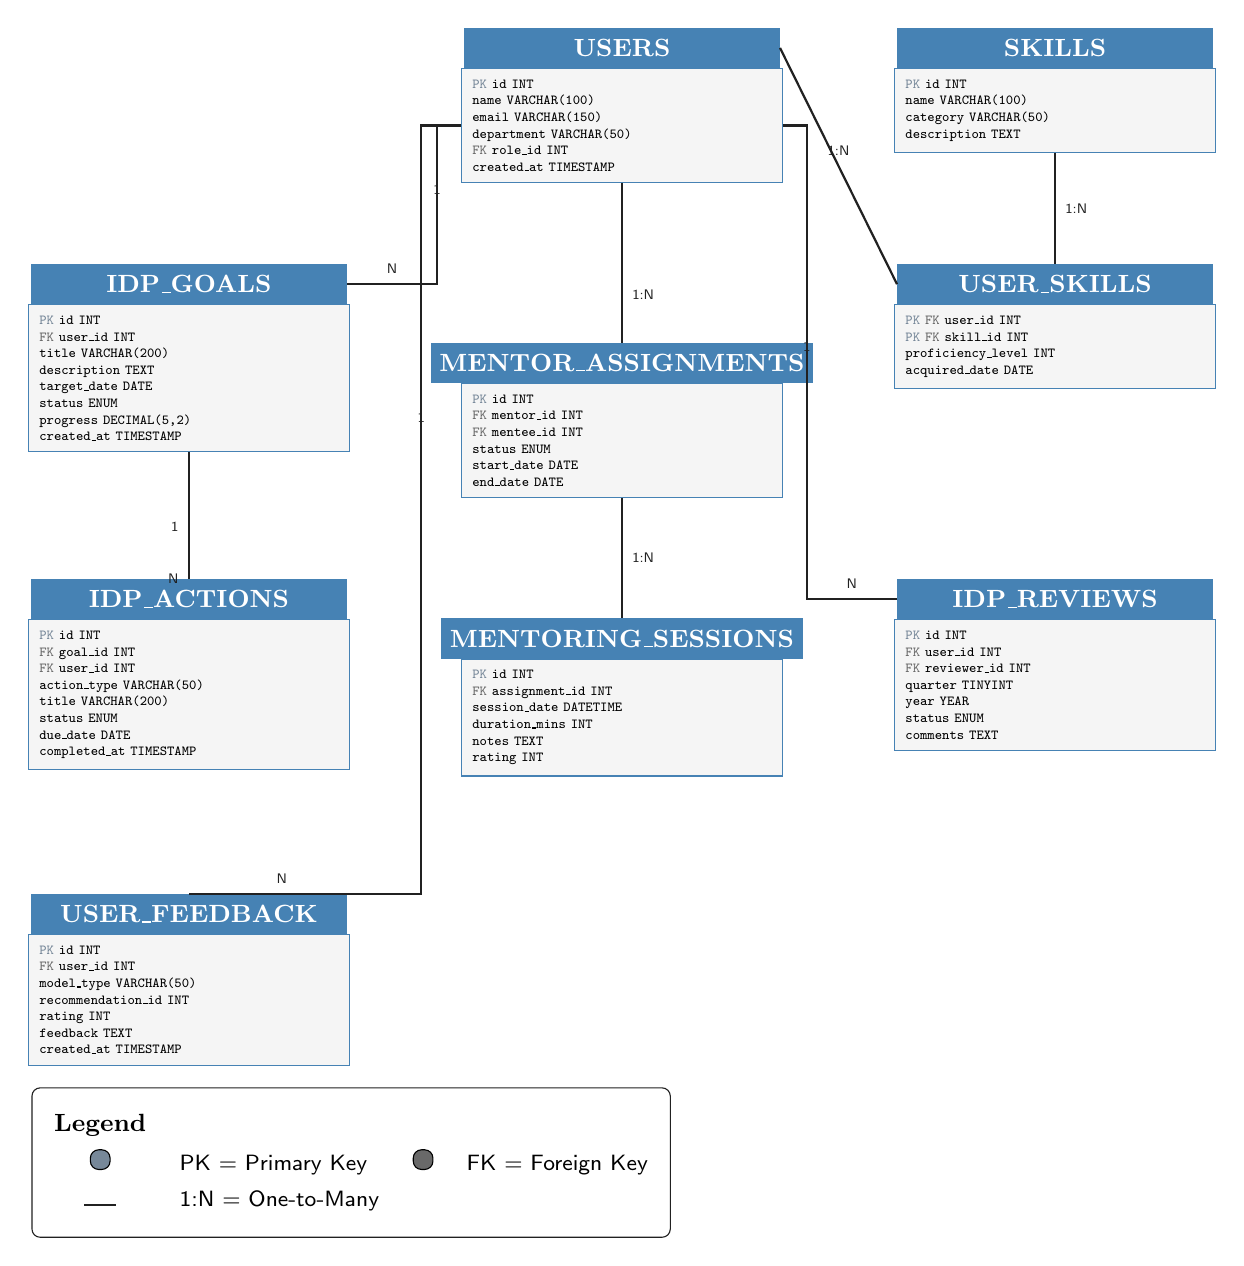
\begin{tikzpicture}[
    % Entity header style
    entityheader/.style={
        rectangle,
        draw=entityHeader,
        fill=entityHeader,
        text=white,
        font=\small\bfseries,
        minimum width=4cm,
        minimum height=0.5cm,
        inner sep=3pt,
    },
    % Entity body style
    entitybody/.style={
        rectangle,
        draw=entityHeader,
        fill=entityBody,
        font=\ttfamily\tiny,
        minimum width=4cm,
        text width=3.8cm,
        inner sep=4pt,
        align=left,
    },
    % Primary key indicator
    pk/.style={text=pkColor, font=\ttfamily\tiny\bfseries},
    % Foreign key indicator  
    fk/.style={text=fkColor, font=\ttfamily\tiny\bfseries},
    % Relationship line
    rel/.style={thick, lineColor},
]

% ============== ENTITIES ==============

% USERS (Central entity)
\node[entityheader] (users_h) at (0, 8) {USERS};
\node[entitybody, anchor=north] (users_b) at (users_h.south) {
    \textcolor{pkColor}{\textbf{PK}} id INT\\
    name VARCHAR(100)\\
    email VARCHAR(150)\\
    department VARCHAR(50)\\
    \textcolor{fkColor}{\textbf{FK}} role\_id INT\\
    created\_at TIMESTAMP
};

% SKILLS
\node[entityheader] (skills_h) at (5.5, 8) {SKILLS};
\node[entitybody, anchor=north] (skills_b) at (skills_h.south) {
    \textcolor{pkColor}{\textbf{PK}} id INT\\
    name VARCHAR(100)\\
    category VARCHAR(50)\\
    description TEXT
};

% USER_SKILLS (Junction table)
\node[entityheader] (userskills_h) at (5.5, 5) {USER\_SKILLS};
\node[entitybody, anchor=north] (userskills_b) at (userskills_h.south) {
    \textcolor{pkColor}{\textbf{PK}} \textcolor{fkColor}{\textbf{FK}} user\_id INT\\
    \textcolor{pkColor}{\textbf{PK}} \textcolor{fkColor}{\textbf{FK}} skill\_id INT\\
    proficiency\_level INT\\
    acquired\_date DATE
};

% IDP_GOALS
\node[entityheader] (goals_h) at (-5.5, 5) {IDP\_GOALS};
\node[entitybody, anchor=north] (goals_b) at (goals_h.south) {
    \textcolor{pkColor}{\textbf{PK}} id INT\\
    \textcolor{fkColor}{\textbf{FK}} user\_id INT\\
    title VARCHAR(200)\\
    description TEXT\\
    target\_date DATE\\
    status ENUM\\
    progress DECIMAL(5,2)\\
    created\_at TIMESTAMP
};

% IDP_ACTIONS
\node[entityheader] (actions_h) at (-5.5, 1) {IDP\_ACTIONS};
\node[entitybody, anchor=north] (actions_b) at (actions_h.south) {
    \textcolor{pkColor}{\textbf{PK}} id INT\\
    \textcolor{fkColor}{\textbf{FK}} goal\_id INT\\
    \textcolor{fkColor}{\textbf{FK}} user\_id INT\\
    action\_type VARCHAR(50)\\
    title VARCHAR(200)\\
    status ENUM\\
    due\_date DATE\\
    completed\_at TIMESTAMP
};

% MENTOR_ASSIGNMENTS
\node[entityheader] (mentors_h) at (0, 4) {MENTOR\_ASSIGNMENTS};
\node[entitybody, anchor=north] (mentors_b) at (mentors_h.south) {
    \textcolor{pkColor}{\textbf{PK}} id INT\\
    \textcolor{fkColor}{\textbf{FK}} mentor\_id INT\\
    \textcolor{fkColor}{\textbf{FK}} mentee\_id INT\\
    status ENUM\\
    start\_date DATE\\
    end\_date DATE
};

% MENTORING_SESSIONS
\node[entityheader] (sessions_h) at (0, 0.5) {MENTORING\_SESSIONS};
\node[entitybody, anchor=north] (sessions_b) at (sessions_h.south) {
    \textcolor{pkColor}{\textbf{PK}} id INT\\
    \textcolor{fkColor}{\textbf{FK}} assignment\_id INT\\
    session\_date DATETIME\\
    duration\_mins INT\\
    notes TEXT\\
    rating INT
};

% IDP_REVIEWS
\node[entityheader] (reviews_h) at (5.5, 1) {IDP\_REVIEWS};
\node[entitybody, anchor=north] (reviews_b) at (reviews_h.south) {
    \textcolor{pkColor}{\textbf{PK}} id INT\\
    \textcolor{fkColor}{\textbf{FK}} user\_id INT\\
    \textcolor{fkColor}{\textbf{FK}} reviewer\_id INT\\
    quarter TINYINT\\
    year YEAR\\
    status ENUM\\
    comments TEXT
};

% USER_FEEDBACK
\node[entityheader] (feedback_h) at (-5.5, -3) {USER\_FEEDBACK};
\node[entitybody, anchor=north] (feedback_b) at (feedback_h.south) {
    \textcolor{pkColor}{\textbf{PK}} id INT\\
    \textcolor{fkColor}{\textbf{FK}} user\_id INT\\
    model\_type VARCHAR(50)\\
    recommendation\_id INT\\
    rating INT\\
    feedback TEXT\\
    created\_at TIMESTAMP
};

% ============== RELATIONSHIPS ==============

% Users -> Goals (1:N)
\draw[rel] (users_b.west) -- ++(-0.3,0) |- node[pos=0.25, above, font=\tiny\sffamily] {1} node[pos=0.75, above, font=\tiny\sffamily] {N} (goals_h.east);

% Goals -> Actions (1:N)
\draw[rel] (goals_b.south) -- ++(0,-0.3) |- node[pos=0.25, left, font=\tiny\sffamily] {1} node[pos=0.75, left, font=\tiny\sffamily] {N} (actions_h.north);

% Users -> Mentor Assignments (1:N as mentor)
\draw[rel] (users_b.south) -- node[pos=0.7, right, font=\tiny\sffamily] {1:N} (mentors_h.north);

% Mentor Assignments -> Sessions (1:N)
\draw[rel] (mentors_b.south) -- node[pos=0.5, right, font=\tiny\sffamily] {1:N} (sessions_h.north);

% Users -> User Skills (1:N)
\draw[rel] (users_h.east) -- node[pos=0.5, above, font=\tiny\sffamily] {1:N} (userskills_h.west);

% Skills -> User Skills (1:N)
\draw[rel] (skills_b.south) -- node[pos=0.5, right, font=\tiny\sffamily] {1:N} (userskills_h.north);

% Users -> Reviews (1:N)
\draw[rel] (users_b.east) -- ++(0.3,0) |- node[pos=0.25, above, font=\tiny\sffamily] {1} node[pos=0.75, above, font=\tiny\sffamily] {N} (reviews_h.west);

% Users -> Feedback (1:N)
\draw[rel] (users_b.west) -- ++(-0.5,0) |- node[pos=0.2, above, font=\tiny\sffamily] {1} node[pos=0.8, above, font=\tiny\sffamily] {N} (feedback_h.north);

% ============== LEGEND ==============
\node[
    draw=lineColor,
    fill=white,
    rounded corners=3pt,
    inner sep=8pt,
    anchor=north west,
    font=\small
] (legend) at (-7.5, -5.2) {
    \begin{tabular}{@{}cl@{\hspace{12pt}}cl@{}}
        \textbf{Legend} & & & \\[3pt]
        \tikz\draw[fill=pkColor] (0,0) rectangle (0.25,0.25); & \textsf{\footnotesize PK = Primary Key} &
        \tikz\draw[fill=fkColor] (0,0) rectangle (0.25,0.25); & \textsf{\footnotesize FK = Foreign Key} \\[2pt]
        \tikz\draw[thick, lineColor] (0,0.1) -- (0.4,0.1); & \textsf{\footnotesize 1:N = One-to-Many} &
        & \\
    \end{tabular}
};

\end{tikzpicture}
\end{document}
